% !TEX root = ./kozhanov_diplom.tex

\documentclass [12pt]{report}
\usepackage [utf8]{inputenc}
\usepackage[T2A]{fontenc}
\usepackage [russianb] {babel}
\usepackage {amsfonts,amssymb,eucal,amsmath,latexsym}
\usepackage{graphics}
\usepackage{array}
\usepackage{multirow}
\usepackage[unicode]{hyperref}

\voffset=-14mm
\textheight=23cm
\linespread{1.3}
\oddsidemargin=5mm
\textwidth=16cm

\usepackage{listings}
\lstloadlanguages{Python}

\begin {document}

\thispagestyle{empty}
\begin{normalsize}
	\begin{center}
		{\bf МИНИСТЕРСТВО ОБРАЗОВАНИЯ РЕСПУБЛИКИ БЕЛАРУСЬ}
	\end{center}

	\begin{center}
		{\bf БЕЛОРУCСКИЙ ГОСУДАРСТВЕННЫЙ УНИВЕРСИТЕТ}
	\end{center}

	\begin{center}
		{\bf Факультет прикладной математики и информатики}
	\end{center}

	\begin{center}
		Кафедра математического моделирования и анализа данных
	\end{center}
\end{normalsize}
\bigskip
\bigskip
\bigskip
\bigskip
\bigskip
\bigskip

\begin{center}
	{\bf Кожановский Василий Николаевич}
\end{center}
\bigskip

\begin{center}
	{\bf ПРИБЛИЖЕННОЕ ВЫЧИСЛЕНИЕ МАТЕМАТИЧЕСКОГО ОЖИДАНИЯ ФУНКЦИОНАЛОВ ОТ ГАУССОВСКОГО ПРОЦЕССА, ОСНОВАННЫХ НА ИНТЕРПОЛЯЦИИ КОРРЕЛЯЦИОННОЙ ФУНКЦИИ}
\end{center}
\bigskip
\bigskip
\bigskip
\bigskip

\begin{center}
	ДИПЛОМНАЯ РАБОТА\linebreak
	студента 5 курса 7 группы
\end{center}
\bigskip
\bigskip
\bigskip
\bigskip

\linespread{1.0}
\begin{tabular}{@{}p{7cm}@{}p{2cm}@{}p{6cm}}
	{\small Допущена к защите} & & {\bf\small Научный руководитель}\\

	\begin{picture}
	    (140,15)\put(0,0){``\line(1,0){20}''\quad\put(0,0){\line(1,0){70}{\small~ 2017 г.}}}
	\end{picture} &  & {\small Егоров Александр Дмитриевич}\\

	{\small Зав. кафедрой математического
	моделирования и анализа данных,
	доктор физ.-мат. наук, профессор,
	чл.-корр. НАН Беларуси Ю. С. Харин } & &
	{\small доктор физико-математических наук,
	профессо, Институт математики НАН Беларуси} \\

\end{tabular}

\vspace{\stretch{1}}
\bigskip
\bigskip
\bigskip
\bigskip
\begin{center}
	\bf{Минск 2017}
\end{center}


\newpage

\begin{center}
	\textbf{РЕФЕРАТ}
\end{center}

\emph{\textbf{Димпломная работа}}, 20 стр.,2 табл., 1 приложение, 5 источников.

\emph{\textbf{Ключевые слова:}} ГАУССОВСКИЕ ПРОЦЕССЫ, ФОРМУЛА ИНТЕРПОЛЯЦИИ, АПРОКСИМАЦИЯ МАТЕМАТИЧЕСКИХ ОЖИДАНИЙ, МАТЕМАТИЧЕСКОЕ ОЖИДАНИЕ, ФУНКЦИОНАЛЫ ОТ ПРОЦЕССА.

\emph{\textbf{Объект исследования}} -- математическое ожидание функционалов от гауссовского процесса.

\emph{\textbf{Цель работы}} -- пременение формулы интерполяции корреляционной функции гауссовского процесса к приближенному вычислению функционалов от процессов.

\emph{\textbf{Методы исследования}} -- методы вычислительной математики, теория случайных процессов.

\emph{\textbf{Результатом}} являются полученные оценки точности метода вычисления мат. ожиданий функционалов.

\emph{\textbf{Областью применения}} является аппроксимация математических ожиданий функционалов от гауссовских процессов.


\newpage

\begin{center}
	\textbf{РЭФЕРАТ}
\end{center}

\emph{\textbf{Дыпломная праца}}, 20 c., 2 табл., 1 дадатак, 5 крыниц.

\emph{\textbf{Ключавыя словы:}}
ГАУСЫВЫ ПРАЦЭСЫ, ФОРМУЛА ІНТЭРПАЛЯЦЫ, МАТЭМАТЫЧНАЕ ЧАКАННЕ, ФУНКЦЫЯНАЛЫ АД ПРАЦЭСУ.

\emph{\textbf{Аб'ект даследавання}} -- матэматычнае чаканне ад гаусавых прасэсаў.

\emph{\textbf{Мэта працы}} -- даследаваць апраксімацыі матэматычных чаканняў функцыяналаў ад рашэнняў стахастычных дыферэнцыяльных раўненняў.

\emph{\textbf{Метады даследавання}} -- метады вылічальнай матэматыкі, тэорыя выпадковых працэсаў.

\emph{\textbf{Вынiкам}} з'яўляюцца атрыманыя ацэнкі дакладнасці метаду вылічэння мат. чакання функцыяналаў.

\emph{\textbf{Bобласцю ўжывання}} з'яўляецца апраксімацыя матэматычных чаканняў функцыяналаў.

\begin{center}
	\textbf{ABSTRACT}
\end{center}

\emph{\textbf{Graduation assignment}}, 2 p., 2 tables, 1 app, 5 sources.

\emph{\textbf{Keywords:}} GAUSSIAN PROCESSES, INTERPOLATION FORMULA , MATHEMATICAL EXPECTATION, FUNCTIONALS.

\emph{\textbf{Research object}} -- mathematical expectation from gaussian processes.

\emph{\textbf{Purpose of the work}} -- explore the approximation of the mathematical expectations of functionals of solutions of stochastic differential equations.

\emph{\textbf{Research methods}} -- methods of computational mathematics, chaotic decomposition.

\emph{\textbf{The result}} is obtained estimates of the accuracy of the method of calculating the math. functional expectations.

\emph{\textbf{Sphere of application }}is approximation of the mathematical expectations of functionals.

\renewcommand\contentsname{Содержание}
\tableofcontents{}

\newpage

\chapter*{Введение}
\addcontentsline{toc}{chapter}{Введение}

Применение приближенных формул к вычислению математических ожиданий
функционалов от гауссовских процессов вида
$ f(x) = \exp\{-\int_{0}^{T}V(x(t))dt\} $
сильно зависит от величины $T. $ Имеющиеся в литературе приближенные формулы
теряют свою эффективность при $T > 1.$
В данной работе рассматривается метод преобразования
математических ожиданий от гауссовского процесса, заданного на $[0;T],$
к математическим ожиданиям от гауссовских процессов, заданных на
промежутках меньшей длины.

Семейство $S$-значных случайных величин $X=(X_t)=(X_t(\omega)), \, t\in [0,T], \, \omega\in \Omega,$ назывется $S$-
\emph{значным случайным процессом}, где $(\Omega,\mathcal{F},P)-$ вероятностное пространство, а $S$ называется
 \emph{фазовым пространством
процесса} $X.$ Если $S=\mathbb{R}^n,$ то процесс называется
$n$-мерным, а если $n=1,$ то процесс называется действительным
случайным процессом. Для действительного случайного процесса
мера в $\mathbb{R}^n,$ определяемая равенством
$$
P_{t_1,\ldots,t_n}(B)\equiv P^X_{t_1,\ldots,t_n}(B)=
P\{\omega\in \Omega:(X_{t_1},\ldots,X_{t_n})\in B\}, \,
B\in \mathcal{B}(\mathbb{R}^n),
$$
назывется \emph{конечномерным
распределением $X.$}
 Наиболее часто конечномерное распределение задается конечномерной функцией распределения процесса
$$
F_{t_1,\ldots,t_n}(u_1,\ldots,u_n)=
P_{t_1,\ldots,t_n}((-\infty,u_1]\times)\ldots\times(-\infty,u_n].
$$
При рассмотрении случайных процессов основным вычислительным соотношением
является
$$
Eg(X_{t_1},\ldots,X_{t_n})=
\int_{\Omega}g(X_{t_1}(\omega),\ldots,X_{t_n}(\omega))dP(\omega)=
\int_{R^n}g(u_1,\ldots,u_n)dF_{t_1,\ldots,t_n}(u_1,\ldots,u_n).
$$
Функция $t\rightarrow X_t(\omega)$ при фиксированном
$\omega\in \Omega$ называется выборочной функцией или траекторией
процесса.

   Процесс называется \emph{непрерывным, непрерывным справа или
слева}, если почти все траектории процесса обладают соответствующим
свойством.

Далее в работе рассматривается гауссовский случайный процесс, функция распределения которого задается плотностью.
Плотность конечномерного распределения гауссовского процесса задаётся равенством:
$$p_{t_1,...,t_n}(u)=
(2\pi)^{-n/2}(\det B)^{-1/2}\exp\Big\{-\frac{1}{2}(B^{-1}(u-m),u-m)\Big\},$$
где $\,B$ -- матрица с элементами $\, b_{ij}=B(t_i,t_j), \,\,i,j=1...n;$
$m=(m(t_1),...,m(t_n)),$ $u=(u_1,\ldots,u_n);$ $\,  B(t,s)\,$ и
$ \,m(t)$ -- заданные функции.
Здесь
$$(B^{-1}(u-m),u-m) = \sum_{k,j=1}^n c_{kj}(u_k-m(t_k))(u_j-m(t_j)),$$
где $\,c_{kj}\,$ - элемент матрицы $\,B^{-1}\,$ обратной к матрице $\,B.$

Равенство (1) в случае гауссовского процесса имеет вид:
$$Eg(X_{t_1},...,X_{t_n})\equiv
\int_{\Omega}g(X_{t_1}(\omega),...,X_{t_n}(\omega)dP(\omega)=
$$
$$
=\int_{R^n}g(u)(2\pi)^{-n/2}(\det B)^{-1/2}
\exp\Big\{-\frac{1}{2}(B^{-1}(u-m),u-m)\Big\}d^n u,
$$
где $d^n u=du_1\ldots du_n.$

Непосредственным вычислением по формуле (2) можно найти, что
$$m(t)=E[X(t)], \qquad B(t,s)=E[(X_t-m(t))(X_s-m(s))].$$
Функции $\,m(t)\,$ и $\,B(t,s)\,$ называются средним значением и
корреляционной функцией гауссовского процесса $X_t.$

Будем предполагать далее, что выборочные функции (траектории) рассматриваемого
гауссовского процесса непрерывны.

  Часто используемым объектом, рассматриваемым в теории гауссовских процессов, является функционал
от траекторий гауссовского процесса. Наиболее простым
объектом такого типа является  функционал вида
\begin{equation}\label{eq:12}
\langle\xi,X\rangle=\int_0^T X_t d\xi(t),
\end{equation}
где $\,\xi=\xi(s)$ -- функция ограниченной вариации.

  В силу непрерывности траекторий
процесса и ограниченности вариации функции $\,\xi\,$, интеграл в правой
части (\ref{eq:12}) существует как интеграл Стилтьеса для всех $\omega\in \Omega$
и имеет место равенство
\begin{equation}\label{eq:13}
\int_0^T X_t d\xi(t)=\lim\limits_{\Delta t\rightarrow 0}
\sum\limits_{k=1}^n X_{t_k}[\xi(t_{k+1})-\xi(t_k)],
\end{equation}
где $t_1\leq t_2\leq\ldots\leq t_n$ -- разбиение отрезка $[0,T];$
$\,\Delta t=\max(t_{k+1}-t_k), k=1,\ldots,n.$

При вычислениях, связанных с гауссовскими процессами, мы будем использовать
следующее равенство
$$(2\pi)^{-n/2}(\det A)^{-1/2}
\int\limits_{R^n}\exp\Big\{-i(u,v)-\frac{1}{2}(A^{-1}u,u)\Big\} d^n u=$$
$$=\exp\Big\{-\frac{1}{2}(Av,v)\Big\},$$
где $A$ -- произвольная невырожденная матрица, $i$ -- мнимая единица.

Для случая $n=1$ эта формула имеет вид:
$$\int\limits_R \exp\{au^2+bu\}du=
\sqrt{\frac{\pi}{-a}}\exp\{-b^2/4a\}.$$

Можно показать, что функционал $\langle\xi,X\rangle$ является гауссовской
случайной величиной. Среднее значение и дисперсию этой величины
можно вычислить с помощью характеристического функционала гауссовского
процесса, определяемого равенством
$$\chi_X(\xi)=E\Big[\exp\Big\{i\langle\xi,X\rangle\Big\}\Big].$$
Используя аппроксимацию (\ref{eq:13}), можно показать, что
\begin{equation}\label{eq:14}
E\Big[\exp\Big\{i\langle\xi,X\rangle\Big\}\Big]=\exp\Big\{
i\int\limits_0^T m(t)d\xi(t)-\frac{1}{2}\int\limits_0^T\int\limits_0^T
B(t,s)d\xi(t)d\xi(s)\Big\}.
\end{equation}

Подставляя в (\ref{eq:14}) $\,\lambda\xi\,$ вместо $\,\xi,\,$ получим равенство
$$E\Big[\exp\Big\{i\lambda\langle\xi,X\rangle\Big\}\Big]=
\exp\Big\{
i\lambda\int\limits_0^T m(t)d\xi(t)-
\frac{\lambda^2}{2}\int\limits_0^T\int\limits_0^T
B(t,s)d\xi(t)d\xi(s)\Big\},$$
из которого следует, что характеристическая функция случайной величины
$\,\langle\xi,X\rangle\,$ является х. ф. гауссовской случайной величины,
имеющей среднее значение и дисперсию
$$m(\xi)=\int\limits_0^T m(t)d\xi(t),\quad
K(\xi,\xi)=\int\limits_0^T\int\limits_0^T
B(t,s)d\xi(t)d\xi(s).$$

Подставляя в (\ref{eq:14}) $\,\sum\limits_{j=1}^n\lambda_j\xi_j\,$ вместо $\,\xi,\,$
получим равенство
$$E\Big[\exp\Big\{i\sum\limits_{j=1}^n\lambda_j\langle\xi_j,X\rangle\Big\}\Big]=
\exp\Big\{
i \sum\limits_{j=1}^n \lambda_j\int\limits_0^T m(t)d\xi_j(t)-$$
\begin{equation}\label{eq:15}
-\frac{1}{2}\sum\limits_{k,j=1}^n\lambda_k\lambda_j\int\limits_0^T\int\limits_0^T
B(t,s)d\xi_k(t)d\xi_j(s)\Big\},
\end{equation}
из которого следует, что характеристическая функция случайного вектора
$\,(\langle\xi_1,X\rangle,\ldots,\langle\xi_n,X\rangle)\,$
является х. ф. гауссовского случайного вектора,
имеющеющего вектор среднего значения и матрицу ковариации с элементами
$$m(\xi_j)=\int\limits_0^T m(t)d\xi_j(t),\quad
K(\xi_k,\xi_j)=\int\limits_0^T\int\limits_0^T
B(t,s)d\xi_k(t)d\xi_j(s). $$
Отсюда следует, что плотность распределения случайного вектора
$\,(\langle\xi_1,X\rangle,\ldots,\langle\xi_n,X\rangle)\,$
имеет вид
$$p_{\xi_1,...,\xi_n}(u)=
(2\pi)^{-n/2}(\det K)^{-1/2}\exp\Big\{-\frac{1}{2}(K^{-1}(u-m),u-m)\Big\},$$
где $\,K$ -- матрица с элементами $\, K(\xi_i,\xi_j), \,\,i,j=1...n;$
$m=(m(\xi_1),...,m(\xi_n)),$ $u=(u_1,\ldots,u_n),$ и имеет место формула
$$E[g(\langle\xi_1,X\rangle,...,\langle\xi_n,X\rangle)]=
\int_{R^n}g(u)p_{\xi_1,...,\xi_n}(u)d^n u.$$
В частности,
$$E[g(\langle\xi,X\rangle)]=
\frac{1}{\sqrt{2\pi K(\xi,\xi)}}\int_{R}g(u)
\exp\Big\{-\frac{1}{2}\frac{(u-m(\xi))^2}{K(\xi,\xi)}\Big\}du.$$

Характеристический функционал (а именно, равенство (\ref{eq:15})) может быть
использован для вычисления моментов:
\begin{equation}\label{eq:20}
E\Big[\prod\limits_{k=1}^{n}\langle\xi_k,X \rangle \Big]=
\frac{1}{i^n}\frac{d^{n}}{d\lambda_1\ldots d\lambda_{n}}
\chi_X \Big(\sum\limits_{k=1}^n\lambda_k\xi_k\Big)
\Big|_{\lambda_1=\ldots =\lambda_{n}=0}.
\end{equation}

Будем полагать в дальнейшем $m(t)=0$ и, следовательно, $m(\xi)=0.$
Тогда
$$E[\langle\xi,X\rangle\langle\eta,X\rangle]=K(\xi,\eta).$$
Пусть далее выполняется условие
\begin{equation}\label{eq:21}
K(\xi,\xi)=0 \quad \text{тогда и только тогда, когда} \,\, \xi=0.
\end{equation}
В силу нашего предположения о непрерывности траекторий процесса,
корреляционная функция $\,B(t,s)\,$ является непрерывной по двум переменным
и, следовательно, удовлетворяет условию
$$
\int\limits_0^T B(t,t)dt\leq\infty,
$$
из которого следует, что ядро $\,B(t,s)\,$ обладает
счетным набором собственных значений и собственных функций
$\lambda_j,$ $\phi_j, \, j=\overline{1,n},$
причем сумма собственных значений конечна:
$$
\sum\limits_{k=1}^{\infty}\lambda_j\leq \infty.
$$
Собственные функции $\phi_j, \, j=\overline{1,n},$ образуют
ортонормированный базис в $L_2([0,T]).$

В случае $\xi_j=\varphi_j(t)=\frac{1}{\sqrt{\lambda_j}}
\int\limits_0^t \phi_j(\tau)d\tau, \,\, j=1,\ldots,n,$ в силу того, что
$$
\int\limits_0^T\int\limits_0^T B(t,s)\varphi_i(t)\varphi_j(s) dtds=\delta_{ij}, \,\,
(K^{-1}u,u)=\sum_{i=1}^{n}u_i^2,
$$
формула (19) преобразуется к виду
\begin{equation}\label{eq:24}
E[g(\langle\varphi_1,X\rangle,...,\langle\varphi_n,X\rangle)]=
\frac{1}{\sqrt{(2\pi)^n}}
\int_{R^n}g(u_1,\ldots,u_n)\exp\Big\{-\frac{1}{2}
\sum_{i=1}^{n}u_i^2\Big\}.
\end{equation}

Имеет место разложение
\begin{equation}\label{eq:25}
X_t=\sum\limits_{k=1}^\infty \langle\varphi_k, X\rangle e_k(t),
\end{equation}
где $e_k(t)=\sqrt{\lambda}\phi_k(t)$, которое
сходится в $sup-$норме пространства $C[0,T]$ для почти всех $\omega\in\Omega.$

Так как $\langle\varphi_k, X\rangle, \, k=1,2,\ldots,$ представляют собой
независимые стандартные гауссовы величины (со средним 0 и дисперсией 1),
для них часто используется обозначение $\xi_k=\langle\varphi_k, X\rangle,$
и тогда ряд (\ref{eq:25}) записывается в виде
\begin{equation}\label{eq:26}
X_t=\sum\limits_{k=1}^\infty \xi_k e_k(t).
\end{equation}
Частный случай такого ряда
\begin{equation}\label{eq:27}
X_t=\sum\limits_{k=1}^\infty \sqrt{\lambda_k}\xi_k \phi_k(t),
\end{equation}
где $\lambda_k, \, \phi_k $ -- собственные значения и собственные функции
ядра $B(t,s),$ называется \emph{разложением Карунена-Лоэва}.


Имеет место следующая формула
\begin{equation}\label{eq:28}
E[f(X_{(\cdot)}+a(\cdot))]=
E[f(X_{(\cdot)})\exp\{a\langle X\rangle-
\frac{1}{2}\|a\|_\mathcal{H}^2\}],
\end{equation}

Далее будут использоваться вариации и производные случайных функционалов, заданных на
траекториях непрерывных гауссовских процессов.\\
Вариация функционала $f(X_{(\cdot)})$ по направлению $a\in\mathcal{H}$
определяется равенством
\begin{equation}\label{eq:29}
\delta_a f(X_{(\cdot)})=\frac{d}{d\lambda}f(X_{(\cdot)}+\lambda a)\Big|_{\lambda=0},
\end{equation}
$$
\delta_{a_1,a_2} f(X_{(\cdot)})=\frac{\partial^2}{\partial \lambda_1 \partial \lambda_2}f(X_{(\cdot)}+\lambda_1 a_1 + \lambda_2 a_2)\Big|_{\lambda_1 = \lambda_2 =0}.
$$
Заметим, что для обычной функции вещественной переменной
$$\delta_a f(u)=
\frac{d}{d\lambda}f(u+\lambda a)\Big|_{\lambda =0}=af'(u), \, u\in R,$$
а для функции n переменных
$$
\delta_a f(u)=\frac{d}{d\lambda}f(u+\lambda a)=
\frac{d}{d\lambda}f(u_1+\lambda_1 a_1,...,u_n+\lambda_n a_n)\Big|_{\lambda = 0}=
$$
\begin{equation}\label{eq:30}
=\sum_{i=1}^n f_{u_i}'a_i=(f'(u),a)_{R^n},
 \,
 \end{equation}
где $f'(u)=grad \, f(u)=
\Big(\frac{\partial f(u)}{\partial u_1},\ldots,
\frac{\partial f(u)}{\partial u_n}\Big),$
$f'_i(u)=\frac{\partial f(u_1,\ldots,u_n)}{\partial u_i}.$

Если найдется такой элемент $f'(X_{(\cdot)})\in V_0[0,T],$ что
$\delta_a f(X_{(\cdot)})=<f'(X_{(\cdot)}),a>,$ то он называется
производной Гато или слабой производной от $f(X_{(\cdot)}).$

Если найдется такой оператор $f''(X_{(\cdot)}): \mathcal{H} \rightarrow \mathcal{H}, $ что
$$
\delta_{a_1, a_2}f(X_{(\cdot)}) = (f''(X_{(\cdot)})a_1,a_2)_{\mathcal{H}},
$$
то $f''(X_{(\cdot)})\equiv f''(X_{(\cdot)})(t,s)$ называется второй производной от $ f(X_{(\cdot)}).$

\underline{Пример.} Пусть $f(\omega)=<\xi,\omega>,$
тогда $\delta_a f = <\xi,a>$ и $f'(x)=\xi.$

Но уже для функционала $a\langle X\rangle$ вариация
$\delta_{a_1}(a\langle X\rangle)=(a_1,a)_\mathcal{H},$
и ясно, что в общем случае не найдется такого элемента $\xi_a,$
что $(a_1,a)_\mathcal{H}=\langle \xi_a,a_1\rangle.$
Таким образом,уже в простых случаях производная Гато не годится
в качестве производной функционалов от случайных процессов.
Подходящим определением является следующее.
 Если существует $f'(X_{(\cdot)})\in\mathcal{H}$ для почти всех $X_{(\cdot)}$
такое, что выполняется равенство
 \begin{equation}\label{eq:31}
 \delta_a f(X_{(\cdot)})=(f'(X_{(\cdot)}),a)_{\mathcal{H}},
 \end{equation}
 то $f'(X_{(\cdot)})$ называется производной $f(X_{(\cdot)})$ по подпространству
 $\mathcal{H}$ или $\mathcal{H}-$производной. Для $f'(X_{(\cdot)})$ используется
 также обозначение  $Df(X_{(\cdot)}).$

Используя равенство (\ref{eq:28}), получим
$$E[\delta_a f(X)]=
 \frac{d}{d\lambda}E[f(X+\lambda a)]\Big|_{\lambda=0}=
 E[f(X)\frac{d}{d\lambda}
 \exp\Big\{\lambda a\langle X\rangle-
 \frac{\lambda^2}{2}\|a\|^2_{\mathcal{H}}\Big\}\Big|_{\lambda=0}],$$
откуда следует
\begin{equation}\label{eq:32}
E[\delta_a f(X)]=E[f(X)a\langle X\rangle].
\end{equation}
Используя (54), а также равенство
\begin{equation}\label{eq:33}
\delta_a(f(X)g(X))=(\delta_a f(X))g(X)+f(X)\delta_a g(X),
\end{equation}
приходим к формуле интегрирования по частям
\begin{equation}\label{eq:34}
E[(\delta_a f(X))g(X)]= E[f(X)g(X)a\langle X\rangle]-E[f(X)\delta_a g(X)].
\end{equation}

Примеры. 1. $D(a\langle X\rangle)=a.$

2. $\delta_{a_1}\langle\xi,X\rangle=\langle\xi,a_1\rangle=
(R\xi,a_1)_\mathcal{H},$
откуда следует
\begin{equation}\label{eq:35}
D(\langle\xi,X\rangle)=R\xi.)
\end{equation}

3. $f(X)=g(a_1\langle X\rangle,\ldots,a_n\langle X\rangle),$
$$
\delta_a f(X)=\sum\limits_{j=1}^n \frac{\partial g}{\partial u_j}
((a_1\langle X\rangle,\ldots,a_n\langle X\rangle)(a,a_j)_\mathcal{H},
$$
$$
Dg(a_1\langle X\rangle,\ldots,a_n\langle X\rangle)=
\sum\limits_{j=1}^n \frac{\partial g}{\partial u_j}
((a_1\langle X\rangle,\ldots,a_n\langle X\rangle)a_j.
$$

\newpage

\chapter{Формула преобразования математического ожидания при интерполяции корреляционной функции}

Для двух гауссовских случайных процесов $X_t,~ t\in[0, T],$
с нулевым средним значением и корреляционными функционалами $K(\xi,\eta)$ и $K_0(\xi,\eta)$ соответственно
определим гауссовкий процесс с корреляционным функционалом
$$
K_u(\xi,\eta)= uK(\xi,\eta)+ (1 - u)K_0(\xi,\eta), u \in [0, 1].
$$
Соответственно для корреляционных функций имеем
$$
B_u(t,s)= uB(t,s)+ (1 - u)B_0(t,s), u \in [0, 1].
$$
Будем предпологать, что эти гауссовские процессы имеют непрерывные траектории,
которые в дальнейшем будем обозначать $X_t = X_t(\omega),~ t \in [0, T],~ \omega \in \Omega.$\

В обычном анализе имеет место следующая формула
\begin{equation}\label{eq:7}
\int_a^b{f(x)p(x)dx} = \int_a^b{f(x)p_0(x)dx} + \int_0^1{\frac{d}{du}}\int_a^b{f(x)p_u(x)dx du},
\end{equation}
где $p_u(x) = up(x) + (1 - u)p_0(x).$ Аналогичная формула имеет место и для математических ожиданий
\begin{equation}\label{eq:8}
E[f(X_{(\cdot)})] = E_0[f(X_{(\cdot)})] + \int_0^1{\frac{d}{du} E_u[f(X_{(\cdot)})] du},
\end{equation}
Из формулы (\ref{eq:8}) следует следующая фомула
\begin{equation}
E[F(X_{(\cdot)})] = E_0[F(X_{(\cdot)})] +
\frac{1}{2}\int_{0}^{1}\int_{0}^{T}\int_{0}^{T}(B(t,s)-B_0(t,s))
E_u[F''(X_{(\cdot)};t,s)]dtdsdu,
\label{eq:1}
\end{equation}
Докажем ее справедливость для функционалов вида
$$
F(X_{(\cdot)}) = \exp\{<\xi,X>\},~~~ \forall \xi \in V[0, T].
$$
Отсюда будет следовать ее справедливость для произвольных
$ F(X_{(\cdot)}) \in L_2(\Phi, P),$ в силу того, что любой функционал
из этого класса опроксимируется линейными комбинациями функционалов вида
$\exp\{<\xi,X>\}.$

Возьмем формулу
\begin{equation}
E[F(X_{(\cdot)})] = E_0[F(X_{(\cdot)})] + \int_{0}^{1}\frac{d}{du}
E_u[F(X_{(\cdot)})]du,
\label{eq:2}
\end{equation}
и применим ее к функционалу $\exp\{<\xi,X>\}.$\\
Имеем в левой части (\ref{eq:2}):
$$
E[\exp\{<\xi,X>\}] = \exp\{
\frac{1}{2}\int_{0}^{T}\int_{0}^{T}B(t,s)d\xi(t)d\xi(s)
\}.
$$
В правой части (\ref{eq:2}):
$$
E_0[\exp\{<\xi,X>\}] = \exp\{
\frac{1}{2}\int_{0}^{T}\int_{0}^{T}B_0(t,s)d\xi(t)d\xi(s)\},
$$
$$
\frac{d}{du}E_u[\exp\{<\xi,X>\}]=\frac{d}{du}\exp\{
\frac{1}{2}\int_{0}^{T}\int_{0}^{T}B_u(t,s)d\xi(t)d\xi(s)\} =
$$
$$
\frac{1}{2}\exp\{
\frac{1}{2}\int_{0}^{T}\int_{0}^{T}B_u(t,s)d\xi(t)d\xi(s)\}
\int_{0}^{T}\int_{0}^{T}\frac{d}{du}
(uB(t,s) + (1-u)B_0(t,s)) d\xi(t)d\xi(s) =
$$
$$
= \frac{1}{2}\exp\{
\frac{1}{2}\int_{0}^{T}\int_{0}^{T}B_u(t,s)d\xi(t)d\xi(s)\}
\int_{0}^{T}\int_{0}^{T}\frac{d}{du}(B(t,s)+B_0(t,s))d\xi(t)d\xi(s)
$$

Вычислим математическое ожидание во втором слогаемом в правой
части равенства (\ref{eq:1}) для функционала
$ F(X_{(\cdot)}) = \exp\{<\xi,X>\}.$
Для этого вычислим сначала
$$
\delta_{a_1,a_2}\exp\{<\xi,X>\} =
\frac{\partial^2}{\partial \lambda_1 \partial \lambda_2}
\exp\{<\xi,X + \lambda_1 a_1 + \lambda_2 a_2>\}
\big|_{\lambda_1=\lambda_2=a}=
$$
$$
= \exp\{<\xi,X>\}<\xi,a_1><\xi,a_2> =
$$
$$
=\int_{0}^{T}\int_{0}^{T}\exp\{<\xi,X>\}a_1(t)a_2(s)d\xi(t)d\xi(s),
$$
откуда следует, что
\begin{equation}\label{eq:6}
(\exp\{<\xi,X>\})''(t,s)=\exp\{<\xi,X>\}\xi(t)\xi(s).
\end{equation}
И далее, так как
$$
E_u[(\exp\{<\xi,X>\})''(t,s)] = E_u[\exp\{<\xi,X>\})]\xi(t)\xi(s)=
$$
$$
=\frac{1}{2}\exp\{\frac{1}{2}
\int_{0}^{T}\int_{0}^{T}B_u(t,s)d\xi(t)d\xi(s)\}\xi(t)\xi(s),
$$
то
$$
\frac{d}{du}E_u[\exp\{<\xi,X>\})]=
\frac{1}{2}\exp\{\frac{1}{2}
\int_{0}^{T}\int_{0}^{T}B_u(t,s)d\xi(t)d\xi(s)\}\times
$$
$$
\times\int_{0}^{T}\int_{0}^{T}(B(t,s)-B_0(t,s))d\xi(t)d\xi(s) =
$$
$$
=\int_{0}^{T}\int_{0}^{T}(B(t,s)-B_0(t,s))
E_u[(\exp\{<\xi,X>\})''(t,s)] dtds,
$$
и далее справедливость форвулы (\ref{eq:1}).


Корреляционную функцию $B_0(t,\tau)$ выберем следующим образом: \\
разобъем область $[0,T]\times[0,T]$ на четыре квадрата
$$
[0,T/2] \times [0, T/2],[0,T/2] \times [T/2, T],[T/2,T] \times [0, T/2],[T/2,T] \times [T/2, T]
$$
и положим $B_0(t,\tau) = B(t,\tau)$ на диагональных квадратах, и $B_0(t,\tau)=0$ вне диагональных квадратов.

Применим формулу (\ref{eq:1}) к математическому ожиданию в правой части этой же формулы:
$$
E[f(X_{(\cdot)})] = E_0[f(X_{(\cdot)})] + \frac{1}{2}\int_0^1\int_0^T\int_0^T{(B-B_0)(t,s)}E_u[f''(X_{(\cdot)};t,s)]dtdsdu =
$$
$$
= E_0[f(X_{(\cdot)})] + \frac{1}{2}\int_0^1\int_0^T\int_0^T{(B-B_0)(t_1,s_1)} E_0[f''(X_{(\cdot)};t_1,s_1)]dt_1ds_1du_1 +
$$
$$
+ \frac{1}{2}\int_0^1\int_0^T\int_0^T{(B-B_0)(t_2,s_2)}\big(
  \frac{1}{2}\int_0^1\int_0^T\int_0^T{(B_{u_1}-B_0)(t_1,s_1)} \times
$$
$$
\times E_{u_1,u_2}[f^{(4)}(X_{(\cdot)};t_1,s_1;t_2,s_2)]dt_1ds_1du_1 \big)
dt_2ds_2du_2
$$
$$
= E_0[f(X_{(\cdot)})] + \frac{1}{2}\int_0^T\int_0^T{(B-B_0)(t_1,s_1)} E_0[f''(X_{(\cdot)};t_1,s_1)]dt_1ds_1 +
$$
$$
+ \frac{1}{2^2}\int_0^1\int_{0}^{1}\int_0^T\int_0^T\int_0^T\int_0^T{u_1(B-B_0)(t_2,s_2)(B-B_0)(t_1,s_1)} \times
$$
$$
\times E_{u_1,u_2}[f^{(4)}(X_{(\cdot)};t_1,s_1;t_2,s_2)]dt_1ds_1
dt_2ds_2du_1du_2.
$$
Продолжая этот процесс итерации $N$ раз, приходим к формуле
\begin{equation}\label{eq:3}
\begin{split}
E[f(X_{(\cdot)})] = \sum_{k=0}^{N}\frac{1}{2^{k}k!}\int_{0}^{T}\stackrel{(2k)}{\cdots}\int_{0}^{T}
\prod_{j=1}^{k}(B-B_0)(t_j, \tau_j)\times \\
\times E[F^{(2k)}(X_{(\cdot)};t,\tau)]d^ktd^k\tau + r_N(F(X_{(\cdot)})),
\end{split}
\end{equation}
где $r_N(F(X_{(\cdot)})) -$ остаток, $t=(t_1,t_2,...,t_k),~ \tau=(\tau_1, \tau_2,...,\tau_k).$

\pagebreak

\chapter{Описание метода апроксимации функционалов от гауссовского процесса, основанного на формуле интерполяции}

Имеет место соотношение
\begin{equation}
E_0[F_{[0,T/2]}(X_{(\cdot)})G_{[T/2,T]}(X_{(\cdot)})]=
E[F_{[0,T/2]}(X_{(\cdot)})]E[G_{[T/2,T]}(X_{(\cdot)})],
\label{eq:4}
\end{equation}
где $F_{[0,T/2]}(X_{(\cdot)}), G_{[T/2,T]}(X_{(\cdot)}) - $
функционалы, зависящие от траекторий процесса $X_t$ на
отрезках $[0,T/2]$ и $[T/2, T]$ соответственно.

Приведем пример, который нам понадобится в последующем. Пусть
$$
F_{[0,T/2]}(X_{(\cdot)}) = \exp\{\int_{0}^{T/2}f(\tau)X_{\tau}d\tau\},
$$
$$
G_{[T/2,T]}(X_{(\cdot)}) = \exp\{\int_{T/2}^{T}g(\tau)X_{\tau}d\tau\}.
$$
Обозначим $\hat{f}(\tau)=f(\tau)$ на $[0, T/2]$
и $\hat{f}(\tau)=0$ на $[T/2, T]$,
$\hat{g}(\tau)=g(\tau)$ на $[T/2, T]$
и $\hat{g}(\tau)=0$ на $[0, T/2]$.
Тогда имеем для данного случая в левой части (\ref{eq:4}):
$$
E_0[F_{[0,T/2]}(X_{(\cdot)})G_{[T/2,T]}(X_{(\cdot)})]=
$$
$$
=E_0[\exp\{\int_{0}^{T/2} f(\tau)X_{\tau}d\tau\}
\exp\{\int_{T/2}^{T} g(\tau)X_{\tau}d\tau\}]=
$$
$$
=E_0[\exp\{\int_{0}^{T}(\hat{f}(\tau)+\hat{g}(\tau))X_{\tau}d\tau\}]=
$$
$$
=\exp\{\frac{1}{2}\int_{0}^{T}\int_{0}^{T}B(\tau_1\tau_2)
(\hat{f}(\tau_1)+\hat{g}(\tau_1))(\hat{f}(\tau_2)+\hat{g}(\tau_2))
d\tau_1\tau_2\}=
$$
$$
= \exp\{\frac{1}{2}\int_{0}^{T/2}\int_{0}^{T/2}B(\tau_1\tau_2)
f(\tau_1)f(\tau_2)d\tau_1\tau_2\} \times
$$
$$
\times \exp\{\frac{1}{2}\int_{T/2}^{T}\int_{T/2}^{T}B(\tau_1\tau_2)
g(\tau_1)g(\tau_2)d\tau_1\tau_2\} \times
$$
$$
\times \exp\{\frac{1}{2}\int_{0}^{T/2}\int_{T/2}^{T}B(\tau_1\tau_2)
\hat{f}(\tau_1)\hat{g}(\tau_2)d\tau_1\tau_2\} \times
$$
$$
\times \exp\{\frac{1}{2}\int_{T/2}^{T}\int_{0}^{T/2}B(\tau_1\tau_2)
\hat{f}(\tau_1)\hat{g}(\tau_2)d\tau_1\tau_2\} =
$$
$\big[~$воспользуемся тем, что
$$
\frac{1}{2}\int_{0}^{T/2}\int_{T/2}^{T}B(\tau_1\tau_2)
\hat{f}(\tau_1)\hat{g}(\tau_2)d\tau_1\tau_2 = 0,
$$
$$
\frac{1}{2}\int_{T/2}^{T}\int_{0}^{T/2}B(\tau_1\tau_2)
\hat{f}(\tau_1)\hat{g}(\tau_2)d\tau_1\tau_2 = 0 ~\big]
$$
$$
= \exp\{\frac{1}{2}\int_{0}^{T/2}\int_{0}^{T/2}B(\tau_1\tau_2)
f(\tau_1)f(\tau_2)d\tau_1\tau_2\}
\exp\{\frac{1}{2}\int_{T/2}^{T}\int_{T/2}^{T}B(\tau_1\tau_2)
g(\tau_1)g(\tau_2)d\tau_1\tau_2\} =
$$
$$
= E[\exp\{\int_{0}^{T/2}B(\tau_1\tau_2)
f(\tau_1)f(\tau_2)d\tau_1\tau_2\}]
E[\exp\{\int_{T/2}^{T}B(\tau_1\tau_2)
g(\tau_1)g(\tau_2)d\tau_1\tau_2\}],
$$
что совпадает с правой частью (\ref{eq:4}).

\chapter{Численные результаты}

В качестве численного примера рассмотрим вычисление математического ожидания фукционала $ \exp\{i\lambda\int_{0}^{T}g(\tau)X_\tau d\tau\} $ от гауссовского процесса с нулевым средним и корреляционной функцией
$B(t,\tau) = \frac{1}{2}\exp(-m|t-\tau|)$
по пространству функций $X=X[0, T]:$
$$
I\equiv I(T) =
E_{[0,T]}[\exp\{i\lambda\int_{0}^{T}g(\tau)X_\tau d\tau\}] =
$$
$$
\exp\Big\{-\frac{\lambda^2}{2}\int\limits_0^T\int\limits_0^T
B(t,s)d\xi(t)d\xi(s)\Big\} =
$$
$$
\exp\Big\{-\frac{\lambda^2}{2}\int\limits_0^T\int\limits_0^T
B(t,s)g(t)g(s)dtds\Big\} =
$$
$$
\exp\Big\{-\frac{\lambda^2}{4}\int\limits_0^T\int\limits_0^T
\exp(-m|t-s|)g(t)g(s)dtds\Big\}.
$$

В рассматриваемом случае
$$
(<\xi,X>)'(t)= g(t),
$$
поскольку имеет место равенство
$<\xi, X> = i\lambda\int_{0}^{T}g(\tau)X_\tau d\tau , $
имеем $ (<\xi,X>)^{(n)}(t)= 0,$ при $ n > 1. $
$$
I(T)\approx \sum_{k=0}^{N}\frac{1}{2^k k!}(i\lambda)^{2k}\times
$$
$$
\times E_{[0,T/2]}[(\int_{0}^{T/2}g(\tau)e^{m\tau}d\tau)^k
\exp\{i\lambda\int_{0}^{T/2}g(\tau)X_\tau d\tau\}]\times
$$
$$
\times E_{[0,T/2]}[(e^{-\frac{mT}{2}}\int_{0}^{T/2}g(\tau)e^{-m\tau}d\tau)^k
\exp\{i\lambda\int_{0}^{T/2}g(\tau)X_\tau d\tau\}]
$$
Для численных расчетов будем пологать $g(t) = e^{-t},$ тогда имеем
$$
I(T)\approx \sum_{k=0}^{N} \frac{(-1)^k\lambda^{2k}} {2^k k!} \times
$$
$$
(\int_{0}^{T/2}e^{-\tau}e^{m\tau}d\tau)^k \times
$$
$$
(e^{-\frac{mT}{2}}\int_{0}^{T/2}e^{-\tau}e^{-m\tau}d\tau)^k
I^2(\frac{T}{2})=
$$

$$
= \sum_{k=0}^{N} \frac{(-1)^k\lambda^{2k}} {2^k k!}
(\int_{0}^{T/2}e^{\tau(m-1)}d\tau)^k \times
$$
$$
(e^{-\frac{mT}{2}}\int_{0}^{T/2}e^{-\tau(m+1)}d\tau)^k
I^2(\frac{T}{2}) =
$$

$$
= \sum_{k=0}^{N} \frac{(-1)^k\lambda^{2k}} {2^k k!}
(\frac{1}{m-1}(e^{\frac{T}{2}(m-1)} - 1))^k \times
$$
$$
(\frac{-1}{m+1}(e^{-\frac{T}{2}(m+1)} - 1) e^{-\frac{mT}{2}})^k
\times I^2(\frac{T}{2}) =
$$

$$
= \sum_{k=0}^{N} \frac{\lambda^{2k}} {2^k k! (m^2 - 1)^k}
(e^{-\frac{T}{2}(m+1)} - 1)^k (e^{-\frac{T}{2}} - e^{-\frac{mT}{2}})^k
I^2(\frac{T}{2}).
$$

Проделав аналогичные вычисления для $(\frac{T}{2})$
и $(\frac{T}{4}),$ получим
$$
I(T)\approx \sum_{k=0}^{N} \frac{\lambda^{2k}} {2^k k! (m^2 - 1)^k}
(e^{-\frac{T}{2}(m+1)} - 1)^k (e^{-\frac{T}{2}} - e^{-\frac{mT}{2}})^k \times
$$
$$
\times[ \sum_{k=0}^{N} \frac{\lambda^{2k}} {2^k k! (m^2 - 1)^k}
(e^{-\frac{T}{2^2}(m+1)} - 1)^k (e^{-\frac{T}{2^2}} - e^{-\frac{mT}{2^2}})^k
]^2 I^{2^2}(\frac{T}{2^2}) \approx
$$

$$
 \approx \sum_{k=0}^{N} \frac{\lambda^{2k}} {2^k k! (m^2 - 1)^k}
(e^{-\frac{T}{2}(m+1)} - 1)^k (e^{-\frac{T}{2}} - e^{-\frac{mT}{2}})^k \times
$$
$$
\times[ \sum_{k=0}^{N} \frac{\lambda^{2k}} {2^k k! (m^2 - 1)^k}
(e^{-\frac{T}{2^2}(m+1)} - 1)^k (e^{-\frac{T}{2^2}} - e^{-\frac{mT}{2^2}})^k
]^2 I^{2^2}(\frac{T}{2^2}) \times
$$
$$
\times [ \sum_{k=0}^{N} \frac{\lambda^{2k}} {2^k k! (m^2 - 1)^k}
(e^{-\frac{T}{2^3}(m+1)} - 1)^k (e^{-\frac{T}{2^3}} - e^{-\frac{mT}{2^3}})^k
]^3 I^{2^3}(\frac{T}{2^3}).
$$

\vspace{1cm}

\noindent Проделав $l$ подобных итераций приходим к выражению

\begin{equation}\label{eq:5}
I(T)\approx \prod_{j=0}^{l-1}(
\sum_{k=0}^{N}\frac{\lambda^{2k}}{2^k k!(m^2 - 1)^{k}}
(e^{-\frac{T}{2^{j+1}}(m+1)} - 1)^k
(e^{-\frac{T}{2^{j+1}}} - e^{-\frac{mT}{2^{j+1}}})^k
)^{2^j} I^{2^l}(\frac{T}{2^l}).
\end{equation}


Вычислим точное значение интеграла $ I(T) = \exp\Big\{-\frac{\lambda^2}{4}
\int_{0}^{T}\int_{0}^{T} e^{-t} e^{-s} e^{-m|t-s|}dtds\Big\}.$ \\
Для этого вычислим сначала
$$
\int_{0}^{T}\int_{0}^{T} e^{-t} e^{-s} e^{-m|t-s|}dtds =
$$
$$
\int_{0}^{T}\int_{0}^{T} e^{-t -s -m|t-s|}dtds =
$$
$$
\int_{0}^{T} \Big[
\int_{0}^{s} e^{-t -s + m(t-s)}dt + \int_{s}^{T} e^{-t -s -m(t-s)}dt
\Big ]ds =
$$
$$
\int_{0}^{T} \Big[
\int_{0}^{s} e^{-t -s + m(t-s)}dt + \int_{s}^{T} e^{-t -s -m(t-s)}dt
\Big ]ds =
$$
$$
\int_{0}^{T} \Big[
\int_{0}^{s} e^{-s(m+1)} e^{t(m-1)} dt + \int_{s}^{T} e^{s(m-1)} e^{-t(m+1)} dt
\Big ]ds =
$$
$$
\int_{0}^{T} \Big[
e^{-s(m+1)} \int_{0}^{s} e^{t(m-1)} dt +  e^{s(m-1)} \int_{s}^{T} e^{-t(m+1)} dt
\Big ]ds =
$$
$$
\int_{0}^{T} \Big[
e^{-s(m+1)} \frac{1}{m-1} e^{t(m-1)} \Big|_{0}^s +
e^{s(m-1)} \frac{-1}{m+1}e^{-t(m+1)} \Big|_{s}^{T}
\Big ]ds =
$$
$$
\int_{0}^{T} \Big[
e^{-s(m+1)} \frac{1}{m-1} (e^{s(m-1)} - 1) +
e^{s(m-1)} \frac{-1}{m+1} (e^{-s(m+1)} - e^{-T(m+1)})
\Big ]ds =
$$
$$
\int_{0}^{T} \Big[
\frac{-1}{m-1} e^{-s(m+1)} + \frac{1}{m-1} e^{-2s} +
\frac{-1}{m+1} e^{s(m-1)} e^{-T(m+1)} + \frac{1}{m+1} e^{-2s)}
\Big ]ds =
$$
$$
\int_{0}^{T} \Big[
\frac{2m}{m^2-1} e^{-2s} +\frac{-1}{m-1} e^{-s(m+1)} +
\frac{-1}{m+1} e^{s(m-1)} e^{-T(m+1)}
\Big ]ds =
$$

$$
= \frac{2m}{m^2-1} (\frac{-1}{2} e^{-2s} \Big|_{0}^{T}) +
\frac{-1}{m-1}( \frac{-1}{m+1} e^{-s(m+1) \Big|_{0}^{T}}) +
$$
$$
+ \frac{-1}{m+1} e^{-T(m+1)} (\frac{1}{m-1} e^{s(m-1)} \Big|_{0}^{T}) =
$$

$$
= \frac{-m}{m^2-1} (e^{-2T} - 1) +
\frac{1}{m^2-1} ( e^{-T(m+1)} - 1) +
$$
$$
+ \frac{-1}{m^2-1} e^{-T(m+1)} (e^{T(m-1)} - 1) =
$$

$$
= \frac{-m}{m^2-1} e^{-2T} + \frac{m}{m^2-1} +
\frac{1}{m^2-1} e^{-T(m+1)} - \frac{1}{m^2-1} -
$$
$$
- \frac{1}{m^2-1} e^{-T(m+1)} e^{T(m-1)} + \frac{1}{m^2-1} e^{-T(m+1)} =
$$

$$
= \frac{-m}{m^2-1} e^{-2T} + \frac{m}{m^2-1} +
\frac{1}{m^2-1} e^{-T(m+1)} - \frac{1}{m^2-1} -
$$
$$
- \frac{1}{m^2-1} e^{-2T} + \frac{1}{m^2-1} e^{-T(m+1)} =
$$

$$
= \frac{1}{m^2-1}( -m e^{-2T} + m +
e^{-T(m+1)} - 1 - e^{-2T} + e^{-T(m+1)} =
$$
$$
= \frac{1}{m^2-1}( 2e^{-T(m+1)} - e^{-2T} (m + 1) + m - 1) =
$$

\noindent Тогда имеем точное значение
$$
I(T) = \exp\{ \frac{- \lambda^2}{4(m^2-1)}
( 2e^{-T(m+1)} - e^{-2T} (m + 1) + m - 1) \}.
$$

\vspace{1cm}

Используем (\ref{eq:5}) для вычисления интеграла $I(\frac{T}{2^l})$.
Результаты вычислений по фурмуле (\ref{eq:5}) для
различных значений $T$ при $\lambda=0.2,~m=2, N=5, l=5$
приведены в следующей таблице:

\begin{center}
\begin{tabular}{ | m{3cm} | m{2cm}| m{2cm} | m{2cm} | m{2cm} | }
\hline
 T & 2 & 4 & 8 & 16 \\
\hline
 точн.знач. & 0.996838 & 0.996675 & 0.996673 & 0.996672 \\
 по ф-ле (\ref{eq:5}) & 0.996845 & 0.996682 & 0.995625 & 0.953672 \\
\hline
\end{tabular}
\end{center}

\noindent При $\lambda=0.5,~m=10, N=10, l=10$
приведены в следующей таблице:
\begin{center}
\begin{tabular}{ | m{3cm} | m{2cm}| m{2cm} | m{2cm} | m{2cm} | }
\hline
 T & 2 & 4 & 8 & 16 \\
\hline
 точн.знач. & 0.994460 & 0.994336 & 0.994333 & 0.994334 \\
 по ф-ле (\ref{eq:5}) & 0.994460 & 0.994335 & 0.994332 & 0.994312 \\
\hline
\end{tabular}
\end{center}

\noindent При $\lambda=0.9,~m=15, N=15, l=15$
приведены в следующей таблице:
\begin{center}
\begin{tabular}{ | m{3cm} | m{2cm}| m{2cm} | m{2cm} | m{2cm} | }
\hline
 T & 2 & 4 & 8 & 16 \\
\hline
 точн.знач. & 0.987685 & 0.987428 & 0.987423 & 0.987423 \\
 по ф-ле (\ref{eq:5}) & 0.987685 & 0.987428 & 0.987422 & 0.987422 \\
\hline
\end{tabular}
\end{center}

\vspace{5mm}

На следующих графиках отображена зависимость погрешности от количества итераций при изменениях параметров $l$ и $N$.

\noindent При $T=16, \lambda=0.5,~m=3, ~N=5, ~l=1...25$ имеем:
\begin{center}
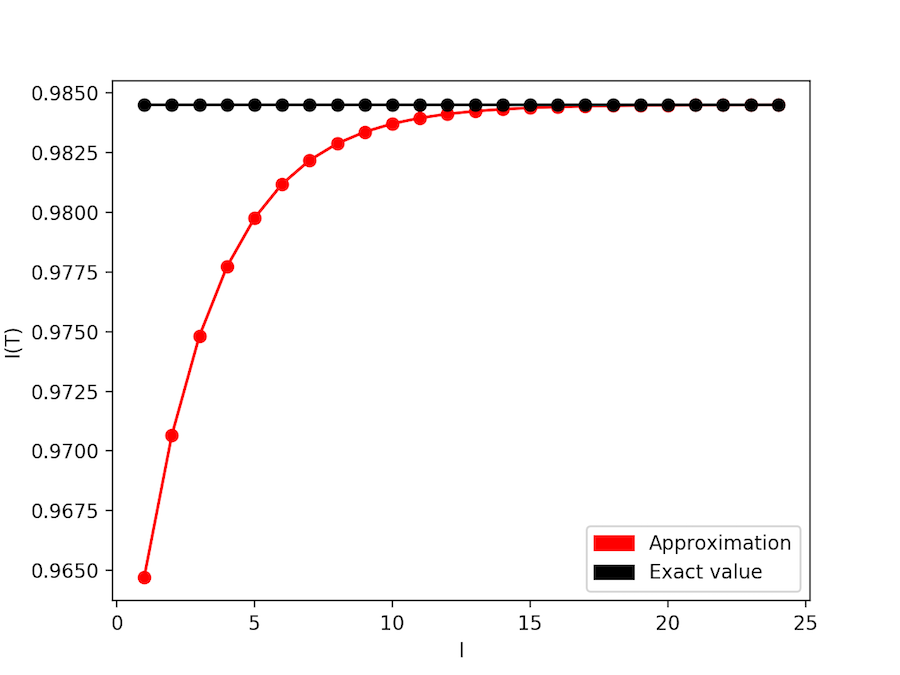
\includegraphics{l_dependency.png}
\end{center}

\noindent При $T=16, \lambda=0.5,~m=3, ~l=2, ~N=1...40$ имеем:
\begin{center}
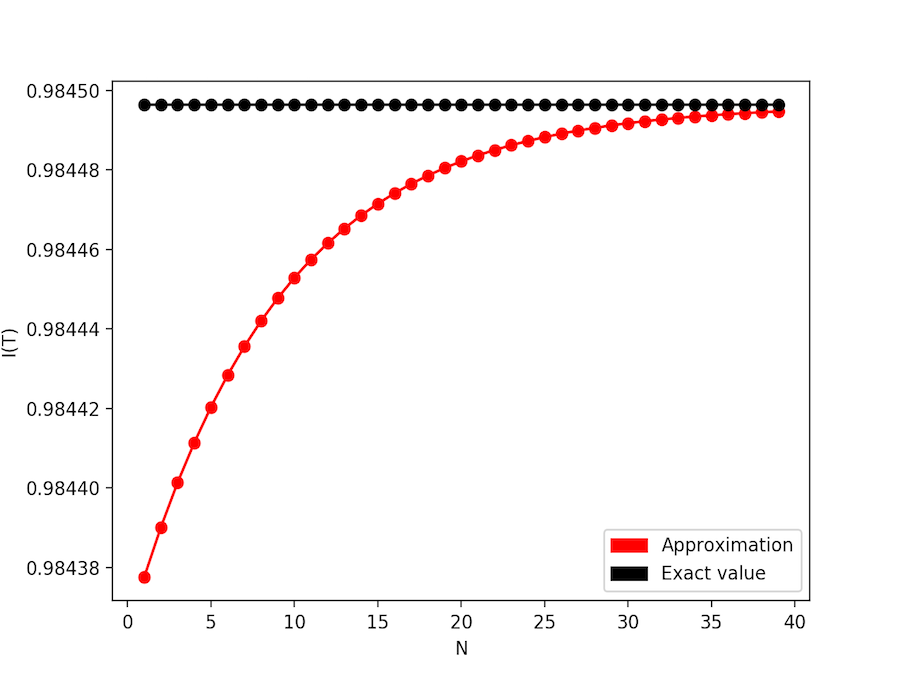
\includegraphics{n_dependency.png}
\end{center}

\chapter*{Приложение 1. Листинг программы}
\addcontentsline{toc}{chapter}{Приложение 1. Листинг программы}

\begin{lstlisting}[language=Python]
#!/usr/bin/python

from math import factorial
from math import exp
from functools import reduce

import matplotlib.patches as mpatches
import matplotlib.pyplot as plot


# exact integral value
def integral_value(t, m):
    e1 = exp(-2. * t)
    e2 = exp(-t * (m + 1.))
    denominator = (m ** 2. - 1.)
    return (2.0 * e2 - e1 * (m + 1.) + m - 1.) / denominator


# accurate value
def exact_value(t, lam, m):
    multiplier = -(lam ** 2.0) / 4.0
    inside = multiplier * integral_value(t, m)
    result = exp(inside)
    return result


# APPROXIMATION
# under sum value calculation
def under_sum(t, lam, m, j: int, k: int):
    numerator = lam ** (2. * k)
    denominator = (2. ** k) * factorial(k) *
    ((m ** 2.0 - 1.0) ** k)
    degree = 2 ** (j + 1)
    e1 = exp(-(m + 1.) * t / degree)
    e2 = exp(-t / degree)
    e3 = exp(-m * t / degree)
    return (numerator / denominator) * (e1 - 1.) **
    k * (e2 - e3) ** k


def sum_value(t, lam, m, n: int, j: int):
    f = lambda s, k: s + under_sum(t, lam, m, j, k)
    result = reduce(f, range(0, n + 1), 0)
    return result


def prod_value(t, lam, m, n: int, l: int):
    f = lambda p, j: p * sum_value(t, lam, m, n, j) ** (2. ** j)
    result = reduce(f, range(0, l), 1.)
    return result


# approximation
# using prod formula
def approximation(t: float, lam, m, n, l):
    prod = prod_value(t, lam, m, n, l)
    exact_t = t / (2. ** l)
    exact = exact_value(exact_t, lam, m) ** (2. ** l)
    return prod * exact


# TESTS
# tests running
def run_test(t, lam, m, n: int, l: int):
    exact = exact_value(t, lam, m)
    approx = approximation(t, lam, m, n, l)
    test_format = "Test with T: %s, lambda: %s, m: %s, N: %s, l: %s"
    print(test_format % (t, lam, m, n, l))
    print("exact value: %.6f" % exact)
    print("approximation: %.6f" % approx)


def test():
    t_values = [
        2.,
        4.,
        8.,
        16.
    ]

    for value in t_values:
        run_test(value, 0.2, 2.0, 5, 5)

    for t in t_values:
        run_test(t, 0.5, 10.0, 10, 10)

    for t in t_values:
        run_test(t, 0.9, 15.0, 15, 15)


def plot_l_dependency():
    n = 5
    m = 3
    t = 16
    lam = 0.5
    exact = exact_value(t, lam, m)

    l_array = range(1, 25)
    values = [approximation(t, lam, m, n, l) for l in l_array]
    exact_values = [exact for l in l_array]

    approx_patch = mpatches.Patch(color='red',
    label='Approximation')
    exact_patch = mpatches.Patch(color='black',
    label='Exact value')
    plot.legend(handles=[approx_patch, exact_patch])

    plot.plot(l_array, values, 'r', l_array, values, 'ro')
    plot.plot(l_array, exact_values, 'k', l_array,
    exact_values, 'ko')
    plot.xlabel('l')
    plot.ylabel('I(T)')
    plot.savefig('l_dependency.png')
    plot.show()

    # linear
    plot.subplot(221)
    plot.plot(x, y)
    plot.yscale('linear')
    plot.title('linear')
    plot.grid(True)

    # log
    plot.subplot(222)
    plot.plot(x, y)
    plot.yscale('log')
    plot.title('log')
    plot.grid(False)


def plot_n_dependency():
    l = 2
    m = 3
    t = 16
    lam = 0.5
    exact = exact_value(t, lam, m)

    n_array = range(1, 40)
    values = [approximation(t, lam, m, n, l) for l in n_array]
    exact_values = [exact for n in n_array]

    approx_patch = mpatches.Patch(color='red',
    label='Approximation')
    exact_patch = mpatches.Patch(color='black',
    label='Exact value')
    plot.legend(handles=[approx_patch, exact_patch])

    plot.plot(n_array, values, 'r', n_array, values, 'ro')
    plot.plot(n_array, exact_values, 'k', n_array,
    exact_values, 'ko')
    plot.xlabel('l')
    plot.ylabel('I(T)')
    plot.savefig('n_dependency.png')
    plot.show()


test()
# plot_l_dependency()
# plot_n_dependency()

\end{lstlisting}


\begin{thebibliography}{99}
\bibitem{lecture} Егоров А.Д. Лекции по стохастическому анализу и его применениям (рукописн.)
\bibitem{wuen} Wuan Luo. Wiener Chaos Expansion and Numerical Solutions of Stohastic Partial Differential Equations / Dissertation (Ph.D.), California Institute of Technology, 2006.
\bibitem{harin} Харин Ю. С. Теория вероятностей, математическая и прикладная статистика: учебник / Ю. С. Харин, Н. М. Зуев, Е. Е. Жук. - Минск: БГУ, 2011. - 463 с.
\bibitem{b1} Егоров А.Д. Введение в теорию и приложения функционального интегрирования / Егоров А.Д., Жидков Е.П., Лобанов Ю.Ю. -
Физмалит: Москва, 2006. - 400 с.
\bibitem{b2} Егоров А.Д. О составной формуле для математического ожидания функционалов от решения уравнения Ито / Вести НАН Беларуси.
Сер.физ.-мат.наук, 2010. №1. С.4-8.
\end{thebibliography}


\end{document}
